\section{Votre première simulation}
%\sectionmark{1\up{ère} sim}
\subsection{Introduction}
Ce chapitre va vous permettre de réaliser une vote première simulation pour la validation de systèmes temps réel en moins de 2 minutes  \smiley ! Voici le résultat que vous obtiendrez au terme : 
\begin{figure}[htbp]
  \centering
  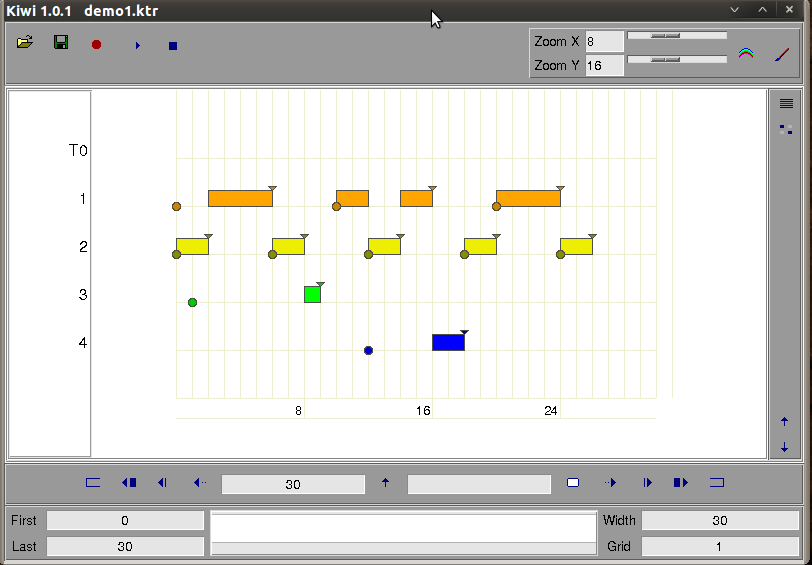
\includegraphics[scale=0.60]{img/RMBG}
  \caption{Votre premier ordonnancement}
  \label{fig:RMtuto}
\end{figure}

\subsection{1\up{ère} Étape : Génération des tâches avec GT} 
\index{Comment commencer}
Dans le dossier GT, entrez la commande suivante \verb+java -jar QT.jar+. On vous propose de choisir entre une génération et une démonstration à partir d'algorithmes pré définis. Tapez 1. On vous propose alors différents algorithmes. Choisissez RMBG. 

\subsection{2\up{ème} Étape : Utilisation de Kiwi}
Si vous ne possédez pas la version de QT incluant Kiwi, ce dernier se lance automatiquement, il ne vous reste plus qu'à cliquez sur le bouton Play. Sinon suivez la démarche suivante :\\ Placez vous dans le dossier ou est installé Kiwi. Tapez la commande suivante  : \verb+./kiwi &+. Une fois dans l'interface de Kiwi, cliquez sur Open. Allez ouvrir votre fichier .ktr se trouvant dans le dossier ou est installé GT. Cliquez sur l'icône Play. \\ Voici le fichier d'ordonnancement que vous être en train de visualiser :  
\begin{verbatim}[htbp]
DECIMAL_DIGITS 0
DURATION 30
LINE_NAME 1 1
LINE_NAME 2 2
LINE_NAME 3 3
LINE_NAME 4 4
PALETTE Rainbow
ZOOM_X 4
ZOOM_Y 16

0 START 1
0 START 2
0 EXEC-B 2

1 START 3

2 EXEC-E 2
2 STOP 2
2 EXEC-B 1

6 EXEC-E 1
6 STOP 1
6 START 2
6 EXEC-B 2

8 EXEC-E 2
8 STOP 2
8 EXEC-B 3

9 EXEC-E 3
9 STOP 3

10 START 1
10 EXEC-B 1

12 EXEC-E 1
12 START 4
12 START 2
12 EXEC-B 2

14 EXEC-E 2
14 STOP 2
14 EXEC-B 1

16 EXEC-E 1
16 STOP 1
16 EXEC-B 4

18 EXEC-E 4
18 STOP 4
18 START 2
18 EXEC-B 2

20 EXEC-E 2
20 STOP 2
20 START 1
20 EXEC-B 1

24 EXEC-E 1
24 STOP 1
24 START 2
24 EXEC-B 2

26 EXEC-E 2
26 STOP 2
\end{verbatim} 


Et voilà avez crée votre première simulation pour la d'un systèmes temps réel  ! Si vous avez rencontrez des difficultés au cours de ce chapitre, vous pouvez vous référer aux différentes parties de ne manuel qui détaille chaque étapes en détail.
